\documentclass[es]{uc3mreport}


\usepackage{import}  % import TeX files
\usepackage{lipsum}  % generates dummy text



% general config

\graphicspath{{img/}}  % Images folder
\addbibresource{references.bib}  % bibliography file

\degree{Bachelor in Computer Science and Engineering}
\subject{Operating Systems}
% \shortsubject{LTX}  % optional
\academicyear{2024-2025}
\group{89}
\author{
          Jorge Adrian Saghin Dudulea -- 100522257
      \\
          Denis Loren Moldovan -- 100522240
      \\
          Antonio Nicolas Lemus Yeguas -- 100522110
      }



\lab{Laboratory 3}
\title{Multi-thread programming}



% report

\begin{document}
    \makecover

    \tableofcontents
    % \listoffigures
    % \listoftables

    % contenidos
    \begin{report}

      % Variable de PANDOC para insertar el contenido del documento
      \part{Description of the code}

      \setcounter{section}{0}

      \setcounter{subsection}{0}

      \setcounter{subsubsection}{0}

      The laboratory is composed of three source files, all compiled
      into the same one. Therefore, multiple header files had been used,
      each one having their respective import protections and function
      declarations.

      \section{queue.c}

      \setcounter{subsection}{0}

      \setcounter{subsubsection}{0}

      This file is responsible for the manipulation of the different
      queues created during the duration of the program. A single queue
      can be used at the same time, following the statement of the
      exercise, therefore, without the need of implementing a more
      complex algorithm to control more queues.

      \subsection{queue\_init}

      \setcounter{subsubsection}{0}

      Function responsible for initializing the queue used by the
      current belt, doing the necessary checks of the input data,
      starting the semaphores and the mutex.

      \subsection{queue\_destroy}

      \setcounter{subsubsection}{0}

      Destroys everything created by the fore mentioned function,
      clearing the remaining elements from the buffer that could not
      have been freed correctly during the belt processing.

      \subsection{queue\_put}

      \setcounter{subsubsection}{0}

      Puts an element into the queue, following the respective
      synchronization mechanisms. For this, three static global
      variables are going to be used, one for the position of the head,
      another for the tail, and the total count of elements inside the
      buffer.

      To calculate the insertion position, we use the operation:

      \[(head\_pos + 1) \% \text{ current\_belt -> size}\]

      Where the head position is the last place where we inserted an
      element, and we perform the modulus with the size of the belt to
      remain inside the belts boundaries.

      \subsection{queue\_get}

      \setcounter{subsubsection}{0}

      As putting an element, we are going to be calculating the position
      of the element to be getting, first retrieving said element from
      the buffer, and then updating the tail position using a similar
      operation as the \texttt{queue\_put} function:

      \[(tail\_pos + 1) \% \text{ current\_belt -> size}\]

      \subsection{queue\_empty}

      \setcounter{subsubsection}{0}

      Checks if the queue is empty by using the \texttt{count} variable.

      \subsection{queue\_full}

      \setcounter{subsubsection}{0}

      Same as \texttt{queue\_empty}, but checks comparing it to the belt
      struct.

      \section{process\_manager.c}

      \setcounter{subsection}{0}

      \setcounter{subsubsection}{0}

      This file contains the code for the threads responsible for
      manufacturing said belts passed as argument to a void pointer. It
      is divided into the manager thread \texttt{process\_manager()},
      the producer and the consumer. All these make use of the queue
      functions.

      \subsection{process\_manager}

      \setcounter{subsubsection}{0}

      Initializes the producer and consumer threads, while parsing the
      input data and synchronizes them with the parent thread from the
      \texttt{factory\_manager}. It is also responsable of creating and
      destroying the belts when the production of elements finishes.

      \subsection{producer}

      \setcounter{subsubsection}{0}

      Produces the elements from the belts, while synchronizing with the
      consumer thread using a mutex to avoid both from modifying the
      belt or the global variables at the same time, and semaphores to
      have extra control over the amount of elements that are being
      produced and the ones that must be retrieved.

      \subsection{consumer}

      \setcounter{subsubsection}{0}

      As already commented in the producer function, uses
      synchronization mechanisms to avoid modifying the belt incorrectly
      and global variables to retrieve the elements.

      \section{factory\_manager.c}

      \setcounter{subsection}{0}

      \setcounter{subsubsection}{0}

      These functions are just responsible from parsing the inputted
      file, checking if the data is correct, and starting starting the
      required threads for running each belt \emph{in order}.

      \subsection{main}

      \setcounter{subsubsection}{0}

      As already mentioned, parses the input file, checks for errors,
      and starts each thread appropriately, while synchronizing with
      them to ensure the correct order. This was the most challenging
      part, as we had to implement multiple semaphores and mutexes to
      guarantee this requirement.

      \subsection{tokenizar\_linea}

      \setcounter{subsubsection}{0}

      Reused function from previous labs, modified to generalize two
      cases of lines to tokenize and improving error management.

      \subsection{parse\_file}

      \setcounter{subsubsection}{0}

      Another reused function, modified to correct a memory leak and
      multiple errors that were arising from not closing the source
      file, therefore leading to undefined behavior.

      \part{Tests}

      \setcounter{section}{0}

      \setcounter{subsection}{0}

      \setcounter{subsubsection}{0}

      When running the tester, there were times when we were getting the
      whole set of tests as correct, and other times when some of them
      were failing. In Debian (Guernika) was less consistent compared to
      Arch (local machine), where we got most of the time the 74/74
      cases. Anyway, we reached to the conclusion that sometimes the
      scheduling of the operating system was putting one of the threads
      before another one, therefore changing the output and failing the
      test. \emph{See Fig. 1}

      \begin{figure}
      \centering
      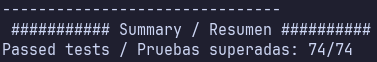
\includegraphics[scale=0.7]{img/tests.png}
      \caption{Tests screenshot}
      \end{figure}

      Aside from the base tests provided in the tester, we are going to
      use the following ones to check manually if the solution follows
      the basic description of the statement.

      \begin{longtable}[]{@{}
        >{\raggedright\arraybackslash}p{(\columnwidth - 6\tabcolsep) * \real{0.1875}}
        >{\raggedright\arraybackslash}p{(\columnwidth - 6\tabcolsep) * \real{0.2708}}
        >{\raggedright\arraybackslash}p{(\columnwidth - 6\tabcolsep) * \real{0.1667}}
        >{\raggedright\arraybackslash}p{(\columnwidth - 6\tabcolsep) * \real{0.3750}}@{}}
      \toprule\noalign{}
      \begin{minipage}[b]{\linewidth}\raggedright
      Test ID
      \end{minipage} & \begin{minipage}[b]{\linewidth}\raggedright
      Description
      \end{minipage} & \begin{minipage}[b]{\linewidth}\raggedright
      Inputs
      \end{minipage} & \begin{minipage}[b]{\linewidth}\raggedright
      Expected Outputs
      \end{minipage} \\
      \midrule\noalign{}
      \endhead
      \bottomrule\noalign{}
      \endlastfoot
      TC01 & Single belt with valid values & Input file:
      \texttt{1\ 1\ 5\ 5} & Producer and consumer complete 5 elements
      successfully \\
      TC02 & Two belts concurrently & Input file:
      \texttt{2\ 1\ 5\ 5\ 2\ 10\ 10} & Both belts produce/consume all
      elements correctly \\
      TC03 & Belt with buffer size 1 & Input file: \texttt{1\ 1\ 1\ 3} &
      Queue operates with minimal size; producer/consumer synchronize
      correctly \\
      TC04 & Belt with zero size (invalid) & Input file:
      \texttt{1\ 1\ 0\ 5} & Error message, program exits with failure \\
      TC05 & Belt with zero elements to produce (invalid) & Input file:
      \texttt{1\ 1\ 5\ 0} & Error message, program exits with failure \\
      TC06 & Belt with negative ID (invalid) & Input file:
      \texttt{1\ -1\ 5\ 5} & Error message, program exits with
      failure \\
      TC07 & Belt with negative size (invalid) & Input file:
      \texttt{1\ 1\ -5\ 5} & Error message, program exits with
      failure \\
      TC08 & Belt with large number of elements & Input file:
      \texttt{1\ 1\ 100\ 1000} & Program runs and processes all elements
      correctly \\
      TC09 & Multiple belts with varied sizes and loads & Input file:
      \texttt{3\ 1\ 5\ 10\ 2\ 3\ 6\ 3\ 7\ 14} & All belts complete
      independently without interference \\
      TC10 & Invalid file with missing fields & Input file:
      \texttt{1\ 1\ 5} & Error message, program exits with failure \\
      TC11 & Queue full scenario handling & Input file:
      \texttt{1\ 1\ 2\ 5} & Producer waits for consumer when queue is
      full, and completes successfully \\
      TC12 & Queue empty scenario handling & Input file:
      \texttt{1\ 1\ 5\ 2} & Consumer waits for producer and completes
      correctly \\
      TC13 & Even belt count mismatch & Input file:
      \texttt{2\ 1\ 5\ 5\ 2\ 10} & Error message, program exits with
      failure \\
      TC14 & File with non-numeric values & Input file:
      \texttt{1\ a\ b\ c} & Error message, program exits with failure \\
      TC15 & Empty input file & Input file: (empty) & Error message,
      program exits with failure \\
      TC16 & Input with extra tokens beyond expected & Input file:
      \texttt{1\ 1\ 5\ 5\ 99} & Error message, program exits with
      failure \\
      TC17 & Producer fails memory allocation & Simulate malloc failure
      in \texttt{producer()} & Error message, thread exits with
      failure \\
      TC18 & Consumer fails integrity check & Simulate mismatch in
      \texttt{id\_belt} & Error message, thread exits with failure \\
      TC19 & Stress test with 100 belts & Input file: \texttt{100}
      followed by 100 belt definitions & All belts process correctly in
      parallel \\
      TC20 & Producer produces only 1 element & Input file:
      \texttt{1\ 1\ 5\ 1} & Single element produced and consumed
      successfully \\
      \end{longtable}

      \part{Conclusion}

      \setcounter{section}{0}

      \setcounter{subsection}{0}

      \setcounter{subsubsection}{0}

      This laboratory helped us understand the important of concurrency
      and synchronization mechanisms, while also teaching us how to
      approach them. The work with the tester is also an important part
      to mention, as it helped us find all the errors that we weren't
      able to acknowledge beforehand.

      To conclude, it was a fascinating exercise, which we are looking
      forward to seeing more in other subjects.

    \end{report}

    
    
\end{document}
